
\section{Protocol Design}
%Unlike the video bit-rate adaptation of FOV-aware streaming, Dante, from the perspective of reliability scheme, preferentially provisions the tiles, viewed by user with higher probabilities and more important to video quality, with more FEC redundancy.  



%We consider the expected video quality loss caused by transmission loss and decoding dependencies of video codec, both of which depend on the FEC parameter adjusting procedure.	
%The core of our system is the FEC adaptation scheme, which is supposed to allocate more redundancy to the data, more closer to the FOV region in order to achieve good video quality as much as possible. But, how to decide which FEC redundancy is optimal is a problem?




\subsection{FEC Redundancy Adaptive Adjusting}
\subsubsection{Optimization Problem}

Obviously, The aim of FEC redundancy adaptation is to minimize the distortion of video viewed by users.
Hence, the problem of FEC redundancy adaptation can be formulated into the following expression of optimization problem.
Given estimated network parameter, such as estimated packet loss rate $\Pi _m^\alpha$, RTT, available bandwidth, the corresponding optimization problem can be formulated as:
\begin{eqnarray}
&{\{ R_m^a\} _{1 \le m \le M,a \in Q}} = \arg \min (\sum\limits_{i = 1}^M {d_{m,effective}}).  \\
&{\rm{subject}}{~~\rm{to}}{~~~T^{tran}} \le {T_{GOP}}~~~~~~~~~~~~~~~~~, \\
&{\rm{and}}{~~~~~~\lambda ^p}(\Phi ) \le {\mu _p}\begin{array}{*{20}{c}}
{}
\end{array}{\rm{}},{\rm{}}~~~~~~~1 \le p \le P~~~,\\
&\begin{array}{*{20}{c}}
{{T^{tran}}{\rm{ = }}}&{\frac{{\sum\nolimits_{m = 1}^M {\sum\nolimits_{\alpha  \in Q} {(V_m^\alpha  \cdot (1 + R_m^a))} } }}{{t{r^{TFRC}}}}}
\end{array},\\
&{\lambda ^p}(\Phi ) = \lambda \frac{{\sum\nolimits_{m = 1}^M {\sum\nolimits_{\alpha  \in Q} {{{(V_m^\alpha  \cdot (1 + R_m^a))}_{_{\left\{ {\Phi _m^\alpha  \in p} \right\}}}}} } }}{{\sum\nolimits_{m = 1}^M {\sum\nolimits_{\alpha  \in Q} {V_m^\alpha } } }}.
\end{eqnarray}

where, the objective function is the minimization of the sum of video distortion for a GOP, subject to constraints of both deadline and available bandwidth. We assume that, the data, from any layer of any frame, makes up an FEC block. The decision variable, \ie output, $\{ R_m^\alpha \}$, is the FEC redundancy of the block for the $\alpha$ layer in the m-th frame. The first constraint (Eq. (3)) indicates that, due to timeliness of video, the data of every GOP should be delivered to the client side before the delay constraint $T_{GOP}$, \ie the transmission time of GOP $T^{tran}$ should be not greater than $T_{GOP}$.
Furthermore, ${V_m^\alpha }$ denotes the size of the $\alpha$ layer for the m-th frame. So, given the packet size, S, the estimated round trip time, RTT and estimated packet loss rate, $\Pi_m^\alpha$, the transmission time of GOP, $T^{tran}$ can be calculated by the size of GOP being divided by the transmission rate, $t{r^{TFRC}}$, according to \cite{TRFC}. 
As for the second constraint, (Eq. (4)) represents the video traffic rate, considering the introduction of FEC redundancy, is supposed to be not greater than available bandwidth.

Therefore, FEC redundancy adaptation can be converted to solving the above optimization problem.

Naturally, we can imagine that, given netowrk parameters, such as estimated packet loss rate, and FEC redundancy, if system of sender side can beforehand calculate quantitatively the quality of video viewed by users of the receiver side, in a somewhat fashion, the FEC redundancy bringing greatest video quality can be a good one.

Fortunately, video distortion computing model can be used to accomplish this. PSNR is used to evaluate video distortion which is calculated via Mean Squared Error (MSE). So, we directly use MSE to denote the video distortion.
In the next, we introduce video distortion computing model, as well as how to beforehand calculate the video distortion.

\subsubsection{The Analysis of Objective Function}
In this section, we focus two things, this first is that, given estimated packet loss rate, how the distortion computing model manifests quantitatively the effect which different FEC redundancy has on the whole distortion?. 
On that basis, the other things is that, since the FOV region which users request can not best completely match the FOV which users finally watch, we need to calculate the quality of video, actually viewed by users, by calculating the expected value of video distortion. 
We next introduce how to mathematically express the the expected value of video distortion. 

According to \cite{distortion_model} and \cite{CMT-VR}, given estimated packet loss rate $\pi _{m}^t$ and FEC redundancy $R_m$,
the distortion of the m-th frame for every video GOP (group of pictures) can be formulated as:${d_m} = d_{m,trunc}(\pi _{m}^t, R_m) + {d_{m,drift}}$. $d_{m,trunc}(\pi _{m}^t, R_m)$ denotes the portion of distortion caused by transmission loss and overdue. ${d_{m,drift}}$ denotes the distortion caused by decoding dependence among frames of video codec. We mainly focus on $d_{m,trunc}(\pi _{m}^t, R_m)$, which is directly related to FEC redundancy.

However, unlike non-360-degree videos, only a small portion of 360-degree videos spatially is perceived by users anytime. Furthermore, according to 360ProbDASH\cite{360ProbDASH}, each tile of 360-degree videos requested by users, is expected to be watched by users with a probability and the probability follows Gaussian Distribution at any time. So we customize the traditional distortion model into the expected value of distortion, called as the effective distortion, which can be calculated via the sum of the distortion of each region being multiplied by its probability of viewing. 
As a result, given estimated packet loss rate $\pi _{m,\alpha }^t$ and FEC redundancy $R_m^\alpha$, each video frame, the effective distortion is formulated as:
\begin{equation}
{d_{m,effective}} = \sum\limits_{\alpha  \in Q} {{\gamma ^\alpha }(d_{m,trunc}^\alpha (\pi _{m,\alpha }^t, R_m^\alpha) + d_{_{m,drift}}^{^\alpha })}
\end{equation}
where Q denotes the layer set of 360-degree videos, which includes FOV layer, cushion layer and outmost layer, as depicted in Figure 3. And given $\alpha $
layer, ${\gamma ^\alpha }$ denotes the accumulated viewing probability of all tiles in the $\alpha$ layer, formulated as:
\begin{equation}
{\gamma ^\alpha } = \sum\limits_{i = 1}^{{\Omega ^\alpha }} {{p_i} \cdot
	{S_i}}
\end{equation}
where ${p_i}$ stands for viewing probability of the i-th tile in the $\alpha $
layer, ${S_i}$ denotes area of the i-th tile and
${\Omega ^\alpha }$ denotes tiles set of the corresponding layer. 

Obvious, the tiles of FOV, requested by users and viewed by users with higher probabilities, are attached with greater weights, \ie accumulated probability, than non-FOV. Thus, improving the distortion of the FOV region can bring more performance gain in video distortion than non-FOV region. 

Meanwhile, in Eq. (7), given the estimated packet loss rate $\pi _{m,\alpha }^t$ and FEC-redundancy rate $R_m^\alpha$, $d_{m,trunc}^\alpha(\pi _{m,\alpha }^t, R_m^\alpha)$ denotes the expected value of MSE for the $\alpha$ layer of the m-th frame, which is
formulated as:
\[d_{m,trunc}^\alpha (\pi _{m,\alpha }^t, R_m^\alpha) = \widehat \delta _m^\alpha  + \Pi _m^\alpha (\pi _{m,\alpha }^t, R_m^\alpha )\cdot\delta _m^\alpha ,1 \le m \le M\]	

where, $d_{m,trunc}^\alpha (\pi _{m,\alpha }^t, R_m^\alpha)$ is proportional to $\Pi _m^\alpha (\pi _{m,\alpha }^t, R_m^\alpha )$. And given a frame $m$, region $\alpha$, FEC-redundancy rate $R_m^\alpha$, and estimated packet loss rate $\pi _{m,\alpha }^t$,
$\Pi _m^\alpha (\pi _{m,\alpha }^t, R_m^\alpha )$ denotes the effective data loss rate, \ie the percentage of lost symbols for the $\alpha$ layer of the m-th frame, caused by transmission loss and expired arrival after the introduction of FEC redundancy,  which is
formulated as:
\begin{small}
\begin{eqnarray}
&\Pi _m^\alpha(\pi _{m,\alpha }^t,R_m^\alpha)  = \left\{ {\begin{array}{*{20}{l}}
{0,\begin{array}{*{20}{c}}
{}
\end{array}if\begin{array}{*{20}{c}}
{\pi _{m,\alpha }^t + (1 - \pi _{m,\alpha }^t)}
\end{array}\cdot\pi _{m,\alpha }^o < \frac{{n - k}}{n},}\\
{\begin{array}{*{20}{c}}
{\pi _{m,\alpha }^t + (1 - \pi _{m,\alpha }^t)}
\end{array} \cdot \pi _{m,\alpha }^o,\begin{array}{*{20}{c}}
{}
\end{array}{\rm{otherwise}}.}
\end{array}} \right.
\end{eqnarray}
\end{small}

where given the $\alpha$ layer of the m-th frames, $(n-k)$ denotes the number of allocated FEC repair packets, $\frac{{n - k}}{n}$ stands for tolerant packet loss rate and $\pi _{m,\alpha }^o$ denotes the overdue loss rate. Obviously, $\Pi _m^\alpha$ is equal to 0 if the provisioning of redundant repair packets is sufficient for countering packet drops caused by transmission loss and expired arrival. 



\subsubsection{An Algorithm To Solve The Optimal Problem}
According to (Eq. 8), the derivation procedure of optimal FEC redundancy can be thought of as the procedure that the system make the effective data loss rate $\Pi _m^\alpha(\pi _{m,\alpha }^t, R_m^\alpha )$ approach the tolerant loss rate $\frac{{n - k}}{n}$.  

Obviously, this require that every FEC repair packet is carefully allocated to each layer of all frames in order to minimize the gap between the $\frac{{n - k}}{n}$ and $\Pi _m^\alpha$. 

we first obtain the mean redundancy of the data in GOP, $R$, from (Eq.2) and (Eq. 3) in order to meet the delay constraint and available bandwidth constraint. And the total number of FEC repair packets, denoted with $A$, is derived via the number of original packets K multiplied by R. Then all the repair packets for one GOP should be allocated into different layers of all frames in the GOP. 
Essentially, this problem is a discrete optimization problem.
It's computational prohibitive to apply the exhaustive search, which should consider all the possible combination of FEC redundancy for all layer of all frame, for the global optimal solution. 
To solve this problem, we design a fast research algorithm, to obtain a sub-optimal solution of FEC redundancy adaptive problem, shown in Algorithm 1. 

\begin{algorithm}[!h] 
	\scriptsize
	\centering 
	\caption{FEC redundancy adaptative algorithm}%算法标题      
	\begin{algorithmic}[1]%一行一个标行号
		\STATE $R = \min (Eq.~(3), Eq.~(4))$ , according to delay constraints, Eq. (3) and
		bandwidth constraints Eq. (4),
		
		\STATE $A = \frac{V}{S} \cdot R$ 
		
		\FOR{$\alpha  \in Q$}  
		
		\STATE Calculate $\gamma ^\alpha$ , according to Eq. (1),
		
		\ENDFOR		
		
		\FOR{$i = 1{\rm{ }} to {\rm{ }}A$}
		\STATE $index{\rm{ }} = {\rm{ }}0,{\rm{ }}{\Delta _d}{\rm{ }} = 0$
		\FOR{$m = 1{\rm{ }}to{\rm{ }}M$}
		\FOR{$\alpha  \in Q$}
		
		\STATE ${d_{effective}} = \sum\limits_{0 \le m \le M} {\sum\limits_{\alpha 
				\in Q} {{\gamma ^\alpha }(d_{_{m,trunc}}^{^\alpha } + d_{_{m,drift}}^{^\alpha
				})} } $
		\STATE ${A_{m,\alpha }} = {A_{m,\alpha }} + 1$
		\STATE $\Delta  = \left| { - {d_{effective}} + \sum\limits_{0 \le m \le M}
			{\sum\limits_{\alpha  \in Q} {{\gamma ^\alpha }(d_{_{m,trunc}}^{^\alpha } +
					d_{_{m,drift}}^{^\alpha })} } } \right|$
		\STATE ${A_{m,\alpha }} = {A_{m,\alpha }} - 1$
		\IF{$\Delta  \ge {\Delta _d}{\rm{ }}$}
		\STATE $index{\rm{ }} = m,\begin{array}{*{20}{c}}
		{layer}
		\end{array} = \alpha ,{\Delta _d} = \Delta$
		\ENDIF
		\ENDFOR 
		\ENDFOR
		\STATE ${A_{index, layer }} = {A_{index, layer }} + 1$
		\ENDFOR
		\RETURN ${\left\{ {{R_{m,\alpha }} = \frac{{{A_{m,\alpha }}}}{{{K_{m,\alpha }}}}} \right\}_{(1 \le m \le M,\alpha  \in Q)}}$
	\end{algorithmic}  
\end{algorithm} 

In Algorithm 1, the aim of line 10 to line 14 is to compare the whole GOP distortion gain after the allocating of one repair packet to one of all possible blocks, which include all layer of all frame in one GOP.  That procedure obtains a local optimal solution each time and as a result, the number of repair packet of the data block, corresponding to the greatest degradation of video distortion, is supposed to be plus one. The complexity of algorithm is $O(N \cdot A \cdot Q)$, and Q is generally equal to 2 or 3.


\subsection{System Overview}

Dante is proposed to support high-quality 360-degree video
streaming service over the wireless network. In Dante, UDP combined with the systematic FEC, RS code, is integrated to provide data delivery service over wireless networks. And only the data of I frames is retransmitted if no ACK is received by the server in time ${T^I}$, in order to guarantee the video data received is decodable by video codec.
Besides, TCP is supplementary to exchange control information, which is of significance. The overall protocol architecture is illustrated in Figure 2.

\begin{figure*}[ht]
	\centering
	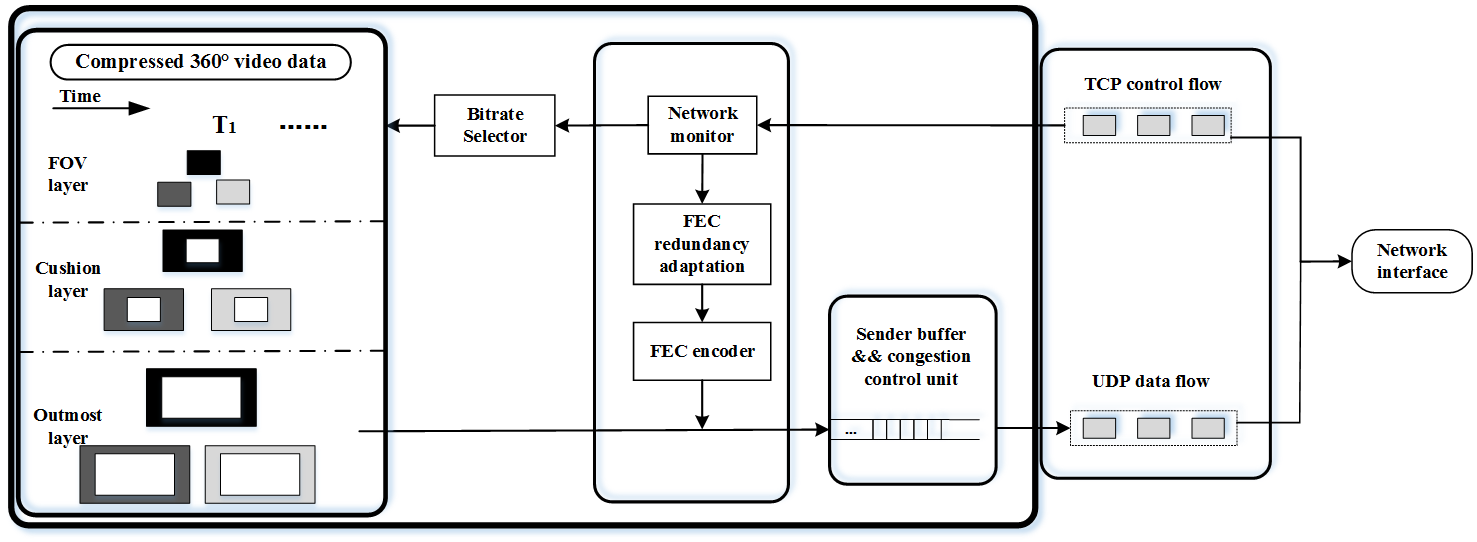
\includegraphics[scale=0.4]{paper_figs/architecture_simple_0624_v7.png}
	\caption{The Architecture of Protocol}
	\label{paper_figs:pathdemo}
\end{figure*}
